% RL-Hammer figure for the ICLR version. Generated by paper/plot_rlhammer.py.
% Mean of two independent attacker runs per target; the shaded band is the per-epoch min/max of those two runs.
% The base-Llama curve averages attacker runs 1 and 3; run 2 collapsed during GRPO training (final ASR 2% against
% 98/99) and is dropped -- state this in the appendix, together with the inference settings.

\begin{figure}[t]
  \centering
  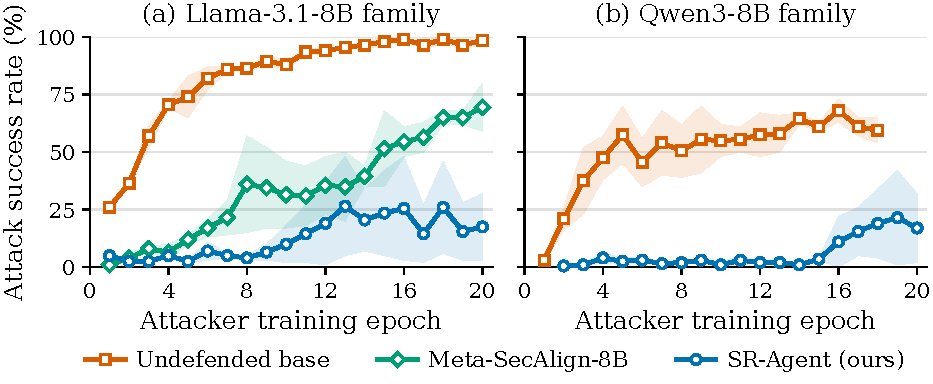
\includegraphics[width=\linewidth]{fig_rlhammer.pdf}
  \caption{Attack success rate (ASR) over attacker training epochs under the RL-Hammer adaptive attack, for
  (a) the Llama-3.1-8B family and (b) the Qwen3-8B family. Each curve is the mean of two independent attacker runs
  against that target, and the shaded band spans the two runs. Lower is better.}
  \label{fig:rlhammer}
\end{figure}
